\section{Ejercicio 8}

\subsection{Introducción}

A fin de realizar un conjunto de experimentos comparativos entre las dos implemetaciones de \textbf{Round Robin}, comenzamos realizando algunas  observaciones.

Se puede ver fácilmente que ambos schedulers tienen exactamente el mismo comportamiento cuando el número de cores es igual a 1, ya que en este caso la cola global del scheduler con migración de tareas (\texttt{RR}) se convierte en su cola local, al igual que en el scheduler sin migración de tareas (\texttt{RR2}). Por consiguiente no es necesario considerar este escenario.

Lo más interesante consiste en considerar para estas pruebas una cantidad de tareas mayor que la cantidad de cores. Asimismo, tomaremos una cantidad de cores $= 3$, un número moderado que nos permitirá evaluar las métricas con facilidad.

Las métricas que utilizaremos para evaluar estos schedulers son \textbf{waiting time} y \textbf{turnaround time}. Aunque en Round Robin estas métricas toman valores intermedios comparadas con otros schedulers, aquí estamos interesados en saber si alguno de \texttt{RR} o \texttt{RR2} minimiza estas métricas.

\subsection{Desarrollo}

%\vspace{1em}
En un esquema con costo de migración $= 0$, intuitivamente es de esperar que el scheduler \texttt{RR} con migración de tareas tenga mejores métricas promedio que el scheduler \texttt{RR2} sin migración. Esto es de suponer ya que el primero mantiene a todos los cores ocupados, mientras que el segundo no ocupará otros cores por más que éstos se encuentren libres cuando las tareas ya fueron asignadas a cores específicos. Para ver esta situación consideremos el lote de tareas siguiente:

\begin{minipage}[t]{0.3\textwidth}
\begin{tarea}[H]
\begin{verbatim}
@0:
TaskCPU 26
TaskCPU 27
@1:
TaskCPU 25
@2:
*2 TaskCPU 30
\end{verbatim}
\end{tarea}
\end{minipage}\\\\

Ejecutando este lote en un procesador de 3 núcleos, con un \textit{quantum} $= 10$ y cambio de contexto $= 0$ obtenemos el comportamiento dado por los siguientes diagramas de Gantt para los scheduler \texttt{RR} y \texttt{RR2} respectivamente:

\begin{figure}[h!t]
  \centering
  \makebox[\textwidth][c]{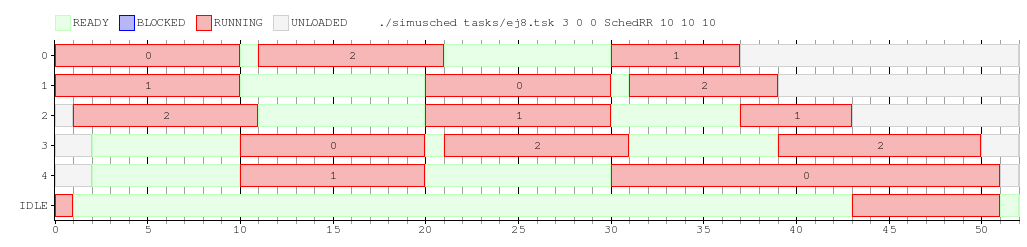
\includegraphics[width=1.2\textwidth]{graphics/ej8-01.png}}%
  \caption{Lote de 5 tareas con \texttt{RR} (costo de migración $= 0$)}
  \label{fig:fig81}
\end{figure}

\begin{figure}[h!t]
  \centering
  \makebox[\textwidth][c]{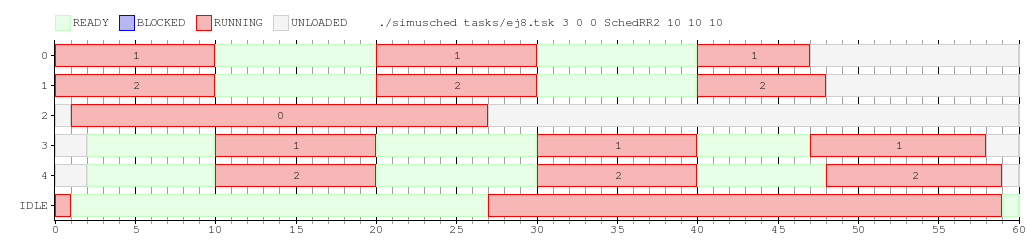
\includegraphics[width=1.2\textwidth]{graphics/ej8-02.png}}%
  \caption{Lote de 5 tareas con \texttt{RR2} (costo de migración $= 0$)}
  \label{fig:fig82}
\end{figure}

\FloatBarrier
En ambos diagramas se puede observar cómo las primeras 3 tareas comienzan a ejecutarse en los 3 cores disponibles. Y en el último diagrama se puede ver cómo las tareas 3 y 4 fueron asignadas a los cores 1 y 2 respectivamente. Sin embargo, puede verse como la tarea 2 se ejecuta exclusivamente en el core 0 hasta que termina. Cuando esto sucede, como las tareas 3 y 4 están asignadas en forma fija a los otros cores, el core 0 queda sin asignación de tareas, y las 4 tareas restantes quedan ejecutándose sólo en 2 cores (el 1 y 2).

Las siguientes tablas muestran el \textbf{waiting time} calculado para cada tarea en ambos schedulers:
\\\\
\begin{tabular}{ll}
\begin{tabular}{ c | c }
  Tarea & Waiting Time \texttt{RR} \\
  \hline
  0 & 10 \\
  1 & 11 \\
  2 & 16 \\
  3 & 17 \\
  4 & 18 \\
\end{tabular}
&
\begin{tabular}{ c | c }
  Tarea & Waiting Time \texttt{RR2} \\
  \hline
  0 & 20 \\
  1 & 20 \\
  2 & 0 \\
  3 & 25 \\
  4 & 26 \\
\end{tabular}
\end{tabular}
\\\\
El promedio para \texttt{RR} es por consiguiente $(10 + 11 + 16 + 17 + 18) / 5 = 14.4$, y para \texttt{RR2} $(20 + 20 + 0 + 25 + 26) / 5 = 18.2$. Como se ve, el promedio para \texttt{RR} es menor. Calculemos asimismo el \textbf{turnaround time} para cada tarea:
\\\\
\begin{tabular}{ll}
\begin{tabular}{ c | c }
  Tarea & Turnaround Time \texttt{RR} \\
  \hline
  0 & 37 \\
  1 & 39 \\
  2 & 42 \\
  3 & 48 \\
  4 & 49 \\
\end{tabular}
&
\begin{tabular}{ c | c }
  Tarea & Turnaround Time \texttt{RR2} \\
  \hline
  0 & 47 \\
  1 & 48 \\
  2 & 26 \\
  3 & 56 \\
  4 & 57 \\
\end{tabular}
\end{tabular}
\\\\
El promedio para \texttt{RR} es $(37 + 39 + 42 + 48 + 49) / 5 = 43$, y para \texttt{RR2} es $(47 + 48 + 26 + 56 + 57) / 5 = 46.8$. El promedio para \texttt{RR} es menor.

Esto coincide con nuestra suposición inicial respecto a este tipo de escenarios. Es decir, siempre que existan cores que hayan quedado libres y todas las tareas ya estén asignadas, se verá un incremento del \textbf{waiting time} y el \textbf{turnaround time} para esas tareas con \texttt{RR2}.
\\\\
Sin embargo, este esquema no es realista, ya que la migración de tareas a otros cores tiene efectivamente un costo asociado. Repitamos las pruebas con el lote anterior pero esta vez con un costo de migración $= 1$:

\begin{figure}[h!t]
  \centering
  \makebox[\textwidth][c]{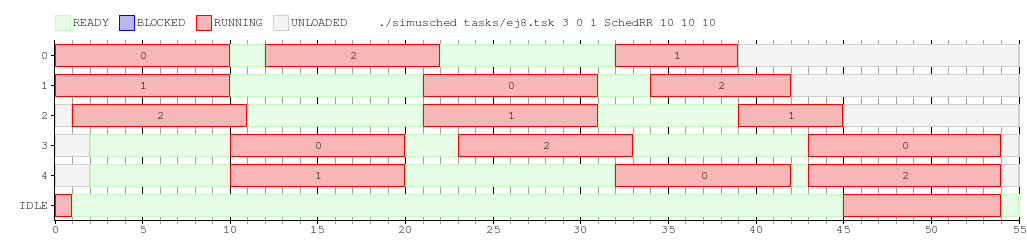
\includegraphics[width=1.2\textwidth]{graphics/ej8-03.png}}%
  \caption{Lote de 5 tareas con \texttt{RR} (costo de migración $= 1$)}
  \label{fig:fig81}
\end{figure}

\FloatBarrier
El gráfico para \texttt{RR2} queda igual que el anterior, por lo que los promedios calculados se mantienen. Calculemos los valores para \texttt{RR}: el promedio de \textbf{waiting time} es $(12 + 14 + 18 + 21 + 21) / 5 = 17.2$, y el de \textbf{turnaround time} es $(39 + 42 + 44 + 53 + 53) / 5 = 46.2$.

Como se puede observar, tanto el \textbf{waiting time} como el \textbf{turnaround time} sigue siendo menor para \texttt{RR}.
Si reiteramos esta prueba con un costo de migración $= 2$ tenemos:

\begin{figure}[h!t]
  \centering
  \makebox[\textwidth][c]{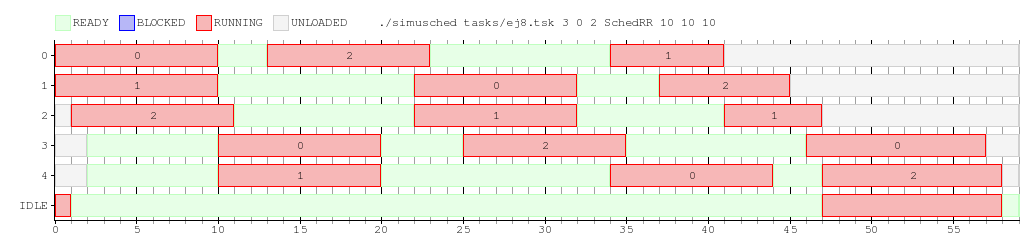
\includegraphics[width=1.2\textwidth]{graphics/ej8-04.png}}%
  \caption{Lote de 5 tareas con \texttt{RR} (costo de migración $= 2$)}
  \label{fig:fig82}
\end{figure}

\FloatBarrier
Calculemos los valores para \texttt{RR}: el promedio de \textbf{waiting time} es $(14 + 17 + 20 + 24 + 25) / 5 = 20$, y el de \textbf{turnaround time} es $(41 + 45 + 46 + 55 + 56) / 5 = 48.6$.
Ya con este costo de migración, tanto el \textbf{waiting time} como el \textbf{turnaround time} es un poco mayor para \texttt{RR}, y seguirá creciendo si seguimos incrementando el costo de migración.

\subsection{Conclusión}

Lo que podemos deducir de este experimento es que si el costo de migración es relativamente bajo en comparación al quantum (su ratio es digamos $\leq \frac{1}{5}$) el scheduler \texttt{RR} expondrá menores tiempos en las métricas usadas en los casos promedio. Si su relación es $> \frac{1}{5}$ entonces el scheduler \texttt{RR2} seguramente comenzará a mostrar mejor desempeño.


